  \chapter{Related Work}
  \label{sec:related-work}

  \section{Scientific Literature}
  \label{subsec:related-scientific-literature}

  \section{Existing Tools and Technologies}
  \label{subsec:related-tools}

    There are many existing tools for model transformations. \citeauthor{kahani2019survey} created a survey in \citeyear{kahani2019survey} of various model transformation tools. They classified 60 different tools, including Henshin. In Figure \ref{fig:tools-environments}, you can see how many tools provide specific execution environments. 73\% of the tools provide plugins for the Eclipse \acs{ide}, and 20\% of the tools are integrated or dependent on other \acsp{ide}. 18\% have no \acs{ide} support, and only two tools are web-based. In total, 89\% of the tools have external dependencies such as an \acs{ide} or other tools. Dependencies often complicate the installation and usage of the tool. \cite{kahani2019survey}

  \begin{figure}[h]
    \centering
    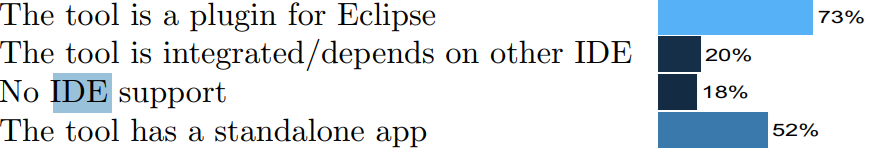
\includegraphics[width=0.6\textwidth]{model-tools.png}
    \caption{Execution environments of model transformation tools. Image obtained from \cite{kahani2019survey}}
    \label{fig:tools-environments}
  \end{figure}

  One web-based tool included in the survey is \ac{atompm} \cite{atompm}. It is a web-based modeling tool to create \ac{dsml} environments, performing model transformations and manipulating and managing models. \cite{atompm} It was created in \citeyear{atompm} and supports all model transformations that are based on T-Core \cite{tcore}, a minimal common basis that allows interoperability between different model transformation languages. \cite{tcore} Metamodels can be defined with a simplified \acs{uml} language. The graphical modeling environment offers debugging and the ability to collaborate and share modeling artifacts in the browser. \cite{atompm}


  There are also other web-based tools for \ac{mde}. WebGME \cite{webGME} is a web-based modeling tool, created in \citeyear{webGME}. It allows to collaboratively design \acp{dsml} using model versioning and broadcasting changes to all active users. It supports prototypical inheritance, where any model can be instantiated recursively, so changes are propagated down the inheritance tree. It also provides scalability, collaborative modeling and model versioning. Metamodels and compositions can be created with WebGME, but no graph transformations can be applied to a model. Even though model transformations are not possible, the editor was one of  the first solutions for web-based modeling tools. \cite{webGME} The software provides extension points to customize or extend the software, but no model transformation capabilities were added by any available extension. \cite{webgme-website} The tool is still hosted and maintained, to be used for free. \cite{webgme-website}


  WebDPF \cite{webDPF} is another web-based modeling tool, published in \citeyear{webDPF}. Compared to WebGME and \ac{atompm}, it supports model navigation and element filter capabilities, a JavaScript editor for writing predicate semantics, reusability of transformation rules, partial model completion, and a termination analysis. These features try to improve the usability of the tool. \cite{webDPF} Even though the tool had improvments upon existing tools, the originally mentioned hosted WebDPF portal is offline by now. 


  There is also a \ac{glsp}-based Ecore metamodel editor, created by the \ac{glsp} development team. It was implemented with the \ac{glsp} version 0.9 but never updated further. It allows to create and edit \ac{emf} Ecore models in a Theia web editor. Even though the project cannot be used directly, due to the use of another source model format and breaking changes in major updates of the \ac{glsp} framework, it provides various classes that can be used as a template for the Henshin Web Ecore viewer. One example is the factory code that maps the \ac{emf} Ecore model to the graphical model. \cite{glsp-ecore-repo}
  The findings show, that there are many existing model transformation tools, but only very few web-based solutions, that provide an easy entry into \ac{mde} and model transformations. Henshin web tries to fill this gap.

  \section{Comparison and Gaps}
  \label{subsec:related-comparison}